\documentclass[usenames,dvipsnames,11pt,pdf,utf8,russian,aspectratio=169]{beamer}
\usepackage{cmap}
\usepackage[T2A]{fontenc}
\usepackage[english,russian]{babel}
\usepackage{subfig}
\usepackage{color}
\usepackage{multicol}
\usepackage{appendixnumberbeamer}
\usepackage{multicol}

\DeclareMathOperator*{\argmin}{arg\,min}

\DeclareMathOperator*{\argmax}{arg\,max}
%
% Choose how your presentation looks.
%
% For more themes, color themes and font themes, see:
% http://deic.uab.es/~iblanes/beamer_gallery/index_by_theme.html
%
\mode<presentation>
{
  \usetheme{Boadilla}      % or try Darmstadt, Madrid, Warsaw, ...
  \usecolortheme{seagull} % or try albatross, beaver, crane, ..

  \usefonttheme{structurebold}  % or try serif, structurebold, ...
  \setbeamertemplate{navigation symbols}{}
  \setbeamertemplate{caption}[numbered]
} 

\captionsetup[subfloat]{labelformat=empty}
\title[Выбор структуры модели]{Байесовский выбор наиболее правдоподобной структуры модели глубокого обучения}
\author{О.\,Ю.\,Бахтеев}


\institute[МФТИ]{Научный руководитель: д.ф.-м.н. В.В. Стрижов\\Московский Физико-Технический Институт (Государственный Университет)}     
%\institute[МФТИ]{Московский Физико-Технический Институт (Государственный Университет)}
\date[2018]{Интеллектуализация обработки информации\\ ИОИ-2018 \\11.10.2018\\}
\begin{document}

\begin{frame}
  \titlepage
\end{frame}


\begin{frame}{Задача выбора структуры модели}
Рассматривается задача регресси или классификации:
\[
    f(\mathbf{x}): \mathbb{R}^n \to \mathbb{Y}, \quad \mathbf{x} \in \mathbf{X}, |\mathbf{X}| = m.
\]

Рассмотрим задачу выбора структуры для однослойной нейросети в задаче классификации:
\[
    f(\mathbf{x}) = \text{softmax}(\mathbf{W}^\text{T}\mathbf{f}_1(\mathbf{x})),
\]
\[
\mathbf{f}_1(\mathbf{x}) = {\gamma}_{0,1}^{1}\mathbf{g}_{0,1}^{1}(\mathbf{x})+\dots+{\gamma}_{0,1}^{K}\mathbf{g}_{0,1}^{K}(\mathbf{x})= {\gamma}_{0,1}^{1}\textbf{tanh}(\mathbf{W}_1^\text{T}\mathbf{x}) + \dots +  {\gamma}_{0,1}^{K}\textbf{tanh}(\mathbf{W}_K^\text{T}\mathbf{x}),
\]
где $\mathbf{W}_1, \dots, \mathbf{W}_K$ --- матрицы одинаковой размерности с различным количеством нулевых строк, $\{\mathbf{g}^{i}_{0,1}\}_{i=1}^K$ --- базовые функции для скрытого слоя нейросети.~\\~\\

\textbf{Структура модели} $\boldsymbol{\Gamma} = [\boldsymbol{\gamma}_{0,1}]$ определяется вершиной булевого $K$-мерного куба.

\end{frame}

\begin{frame}{Задача выбора структуры модели: усложненный пример}
Рассмотрим задачу выбора структуры для однослойной нейросети с неизвестной функцией активации:
\[
    f(\mathbf{x}) = \text{softmax}(\mathbf{W}^\text{T}\mathbf{f}_{K+1}(\mathbf{x})),
\]
\[
\mathbf{f}_{K+1}(\mathbf{x}) =  {\gamma}_{1,K+1}\mathbf{g}_{1,K+1}(\mathbf{x})+\dots+{\gamma}_{K,K+1}\mathbf{g}_{K,K}(\mathbf{x})=  {\gamma}_{1,K+1}\mathbf{f}_1(\mathbf{x})+\dots+{\gamma}_{K,K+1}\mathbf{f}_{K}(\mathbf{x}),
\]
\[
    \mathbf{f}_i(\mathbf{x}) =  {\gamma}_{0,i}^{1}\mathbf{g}_{0,i}^{1}(\mathbf{x})+{\gamma}_{0,i}^{2}\mathbf{g}_{0,i}^{2}(\mathbf{x}) = {\gamma}_{0,i}^{1}\textbf{tanh}(\mathbf{W}_{i}^\text{T}\mathbf{x})+{\gamma}_{0,i}^{2}{\sigma}(\mathbf{W}_{i}^\text{T}\mathbf{x}), \quad i=1,\dots K.
\]

\textbf{Структура модели} $\boldsymbol{\Gamma} = [\boldsymbol{\gamma}_0, \dots, \boldsymbol{\gamma}_{K+1}] $ определяется вершиной булевого $K$-мерного куба.

\end{frame}


\begin{frame}{}
Пример для более сложной структуры.
Сложная нейросеть.
\end{frame}


\begin{frame}{Выбор  структуры модели: базовые определия}
\begin{itemize}
\item \textbf{Модель глубокого обучения --- } суперпозиция дифференцируемых функций.
\item Качество модели определяется \textbf{параметрами} модели.
\item Оптимизация параметров определяется \textbf{гиперпараметрами и структурными параметрами} модели.
\item \textbf{Гиперпараметры} --- параметры распределения параметров модели.
\item \textbf{Структурные параметры} --- параметры, определяющие структуры модели.
\end{itemize} 
\end{frame}


\begin{frame}{Выбор  структуры модели глубокого обучения}

\textbf{Цель работы:}\\
Развитие теории исследования метода байесовскогго выбора модели глубокого обучения
\textbf{Задачи:}
\begin{itemize}
\item Предложить алгоритм оптимизации параметров, гиперпараметров и структурных параметров моделей глубокого обучения.
\item Предожить метод выбора ниболее правдоподобной структурной модели.
\item Исследовать свойства оптимизационных алгоритмов выбора модели.
\end{itemize}
\textbf{Основные проблемы}
\begin{itemize}
\item Многоэкстремальность задачи оптимизации параметров модели.
\item Вычислительная сложность оптимизации.
\item Большое количество параметров и гиперпараметров.
\end{itemize}

\end{frame}


\begin{frame}                                                                                                                                   
\frametitle{Проблемы обучения сетей}                                                                                                          
Правдоподобие моделей с избыточным количеством параметров не меняется при удалении параметров.                                                       
\begin{figure}[h]                                                                                                                               
\centering                                                                                                                                      
\subfloat[Избыточность параметров модели]{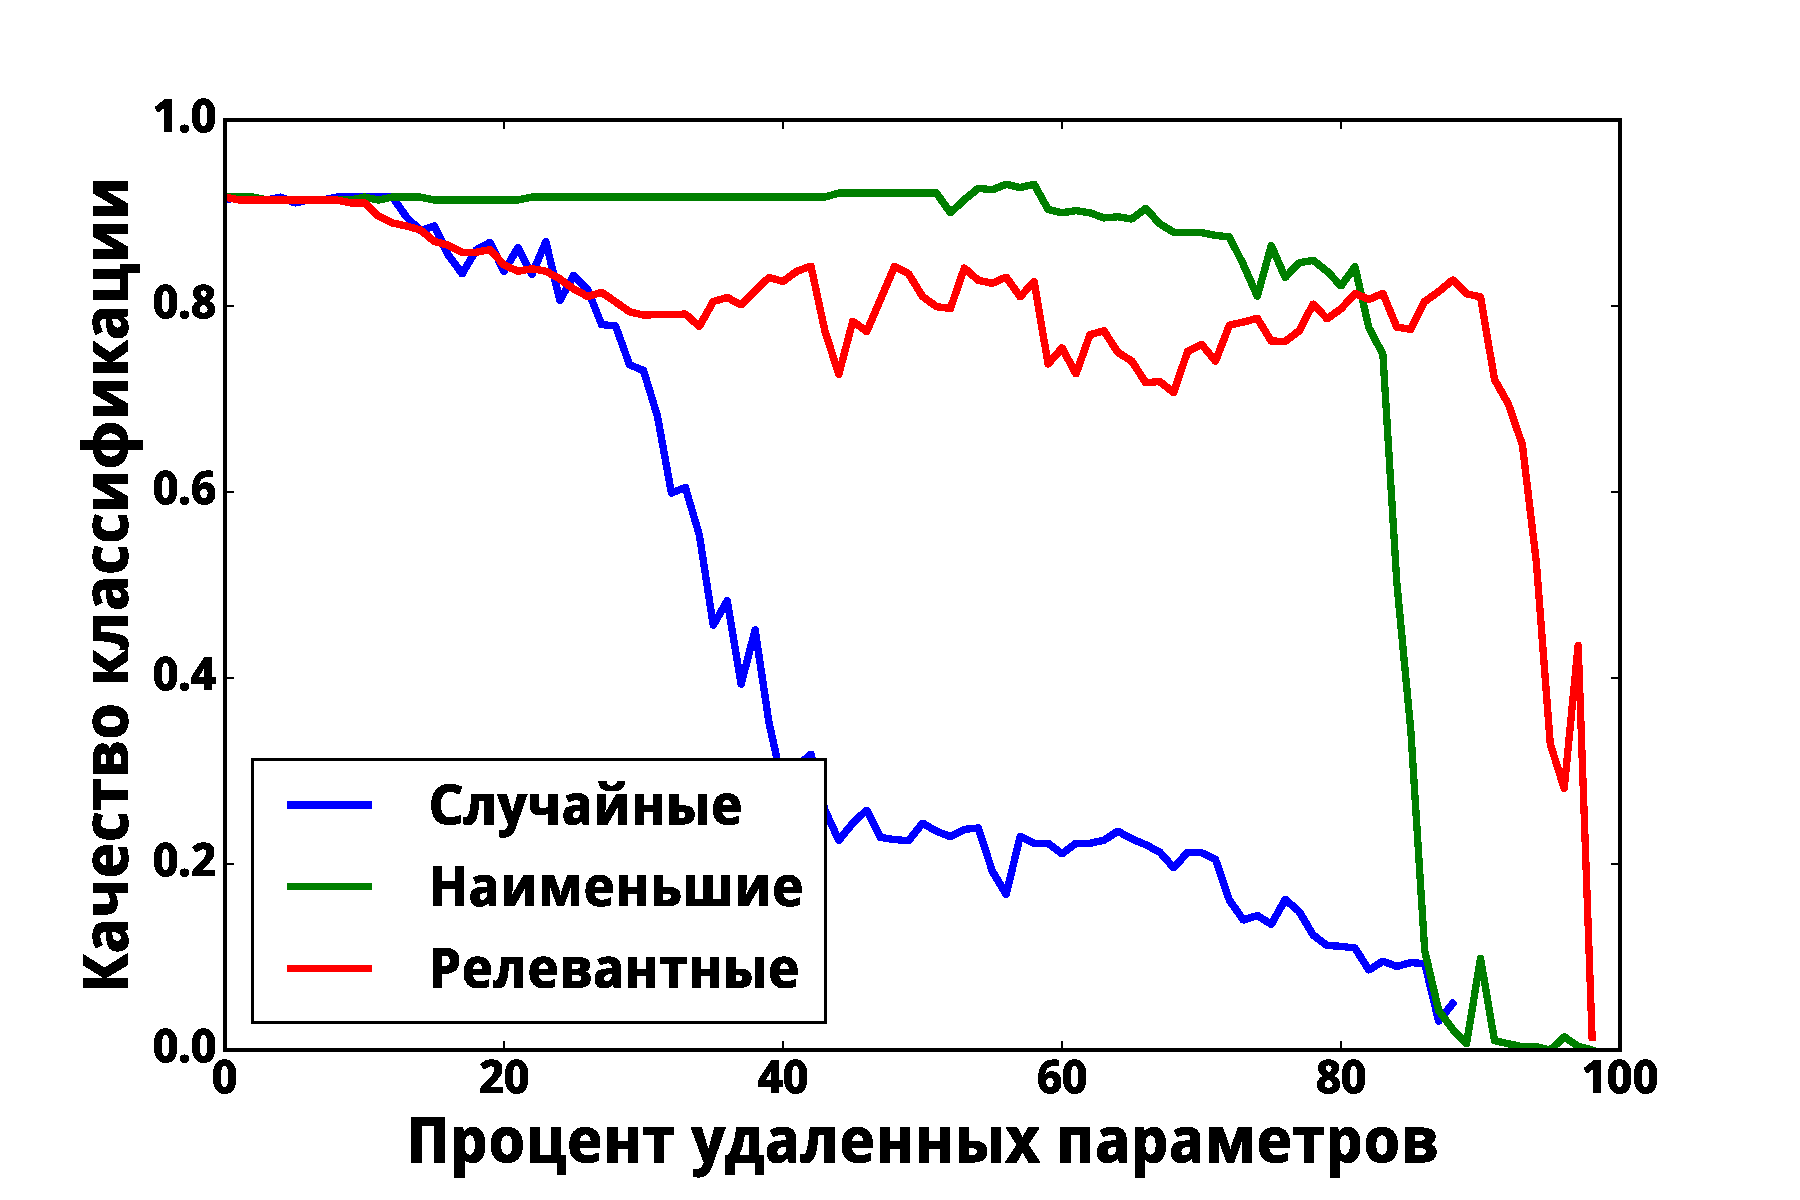
\includegraphics[width=0.45\textwidth]{./slide_plots/pruning.pdf}}                                          
\subfloat[Неустойчивость модели]{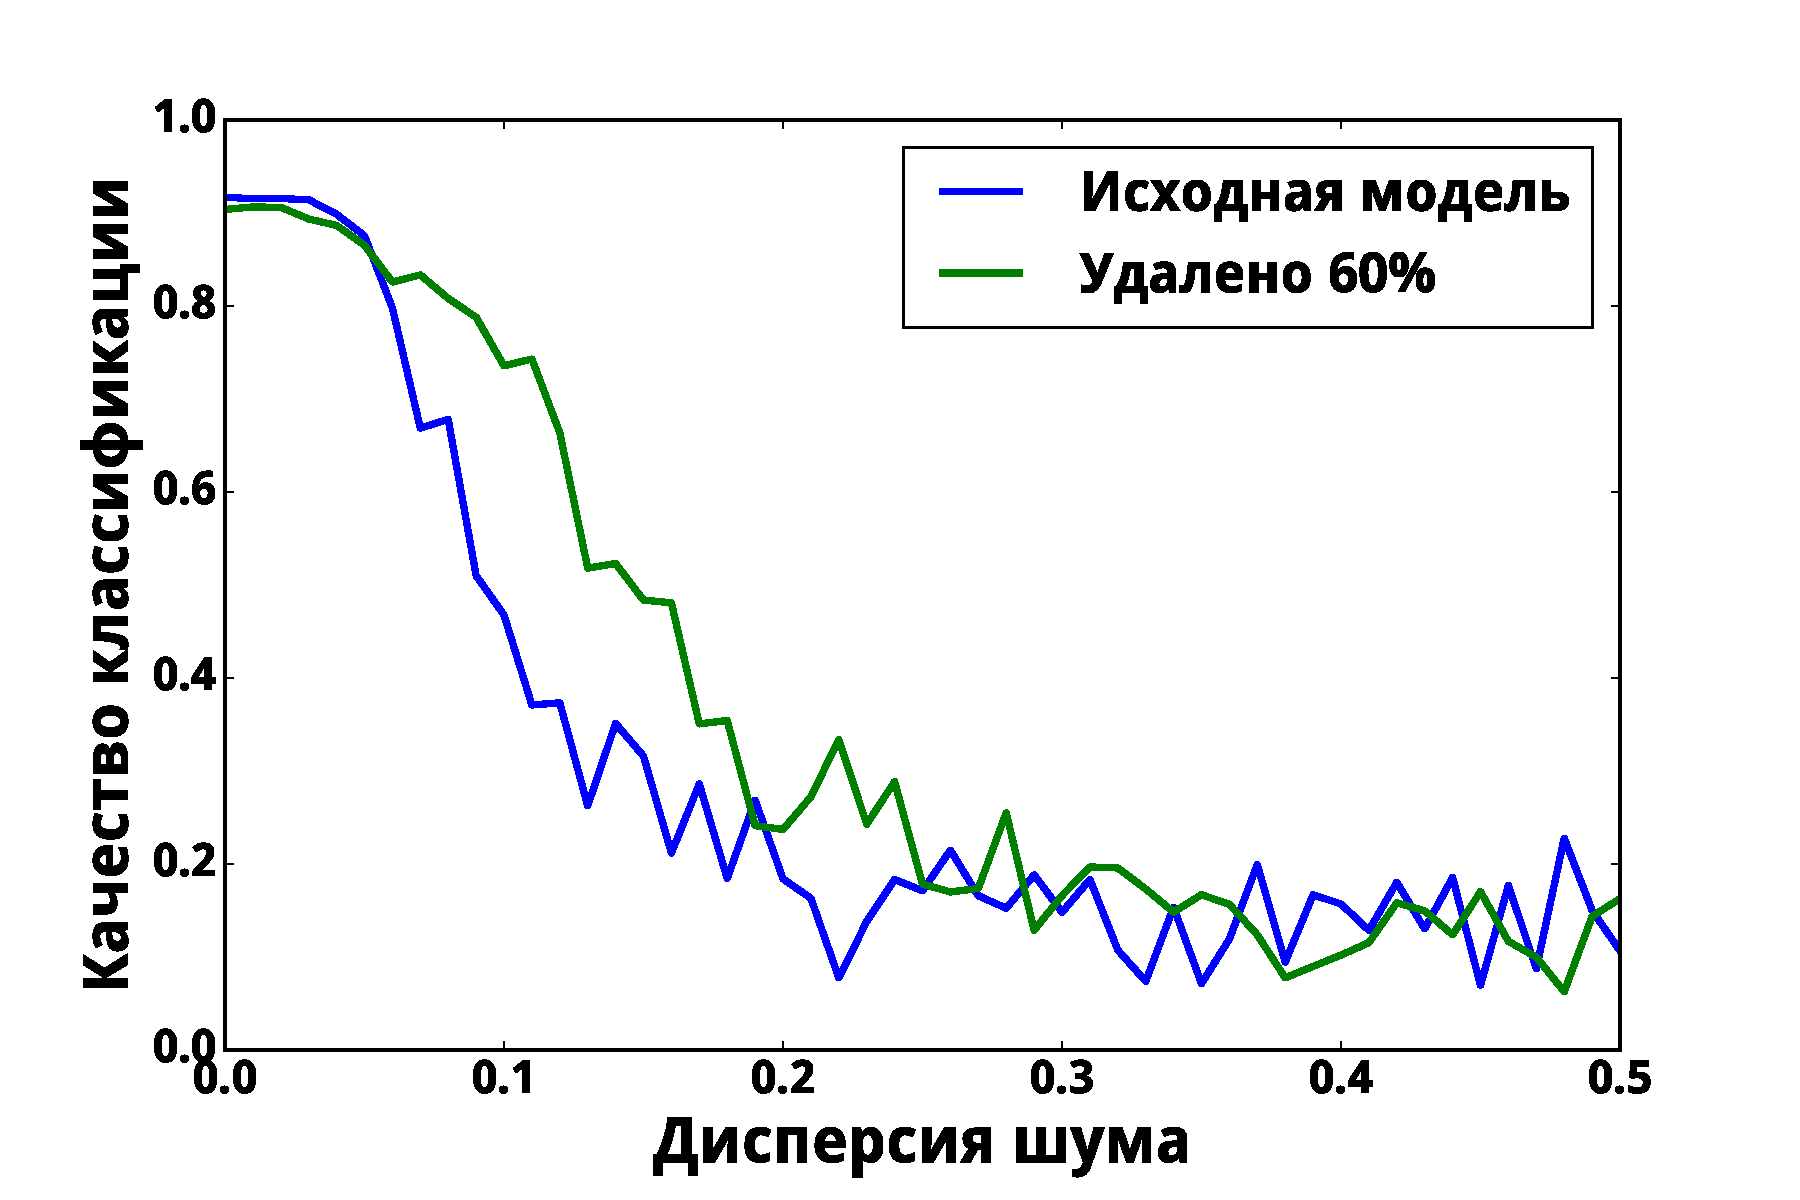
\includegraphics[width=0.45\textwidth]{./slide_plots/noise.pdf}}                                                     
\end{figure}                                                                                                                                    
                                                                                                                                                
\end{frame}    




\begin{frame}{Правдоподобие модели}  
                                                                                          
Пусть заданы априорное распределение параметров и структуры $p(\mathbf{W}, \boldsymbol{\Gamma})$.

Модель $\mathbf{f}$  оптимальна, если достигается максимум \textbf{правдоподобия модели}:                                      
\[                                                                                                                                              
        p(\mathbf{y}|\mathbf{X}) = \int_{\mathbf{W}, \boldsymbol{\Gamma} } \textcolor{red}{p(\mathbf{y}|\mathbf{X},\mathbf{W},  \boldsymbol{\Gamma})} \textcolor{blue}{p(\mathbf{W}, \boldsymbol{\Gamma}) d\mathbf{W}d{\boldsymbol{\Gamma}}}.                         
\]       


\begin{figure}
  \centering
 \subfloat[Схема выбора модели по правдоподобию]{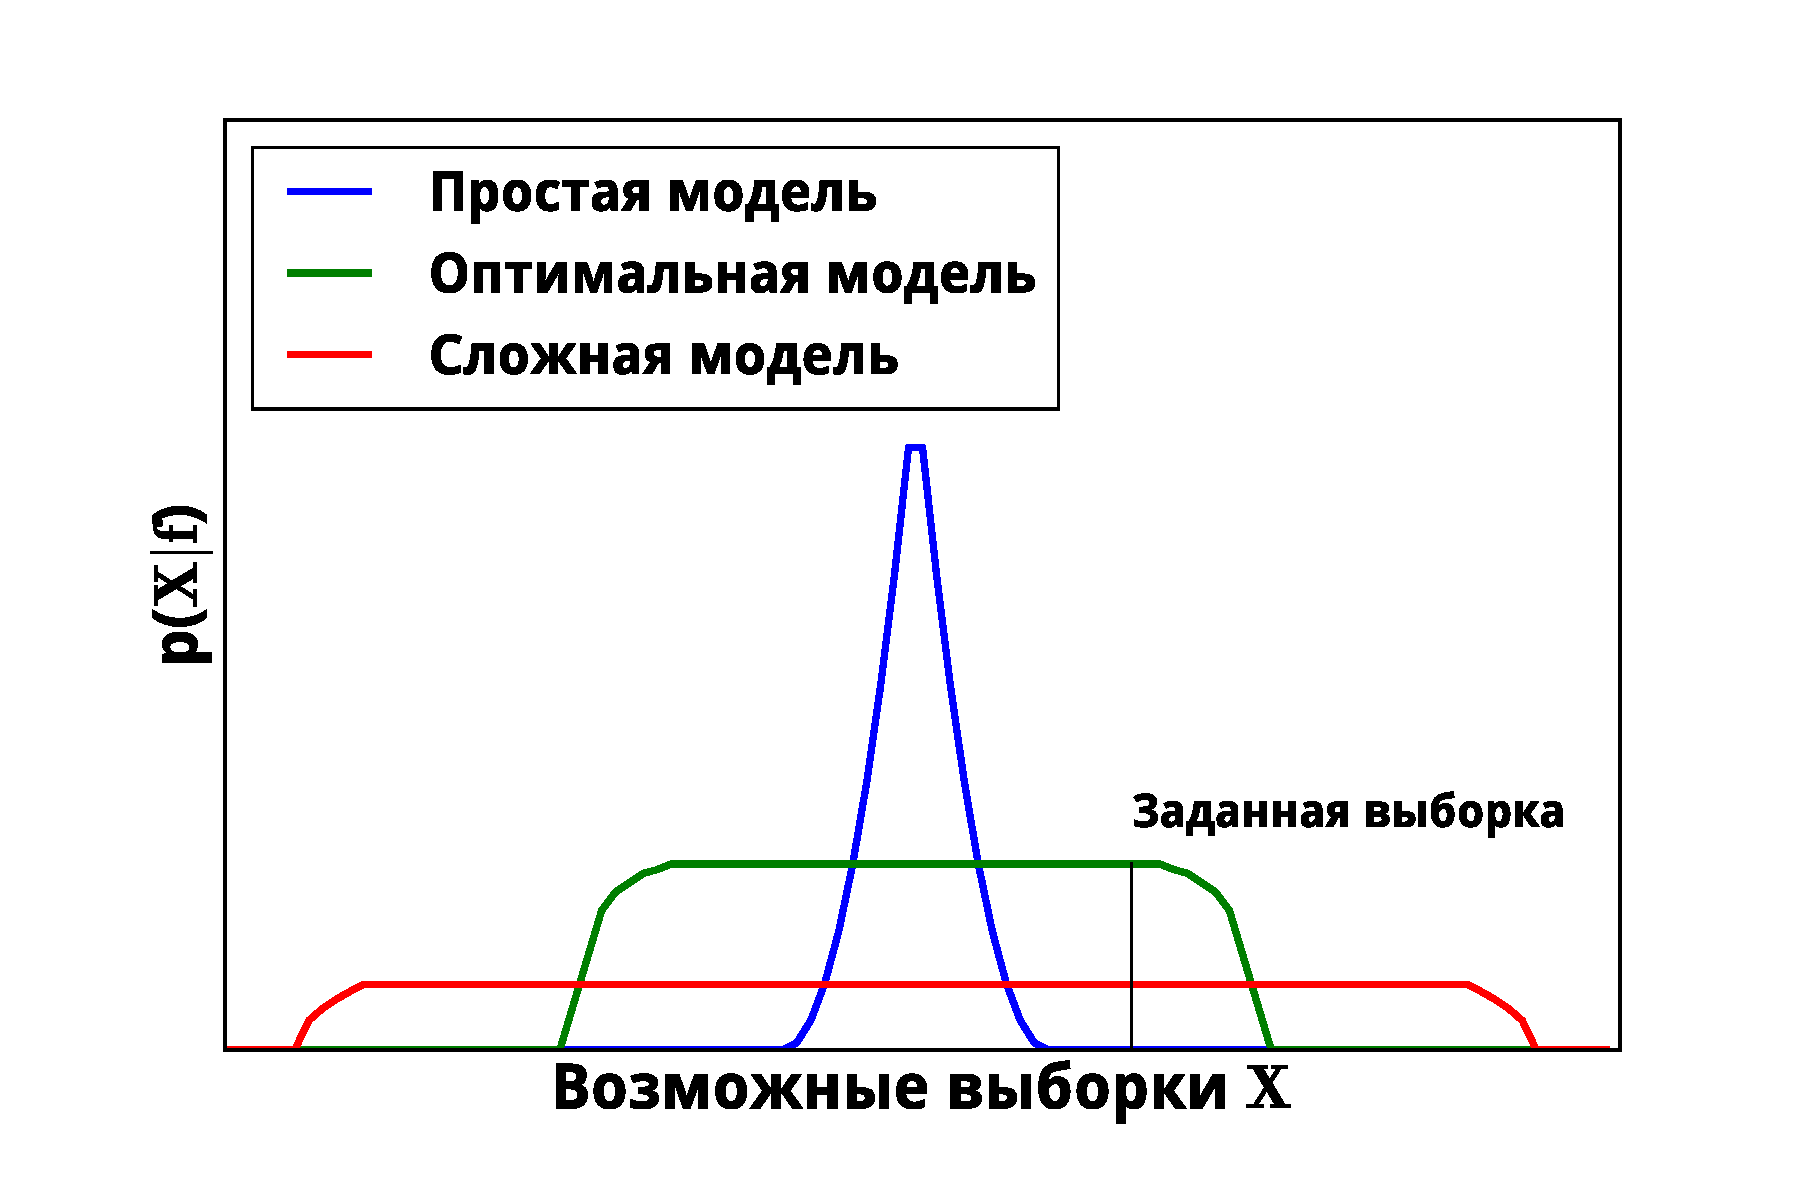
\includegraphics[width=0.4\textwidth]{slide_plots/evidence.pdf}} 
 \subfloat[Пример: полиномы]{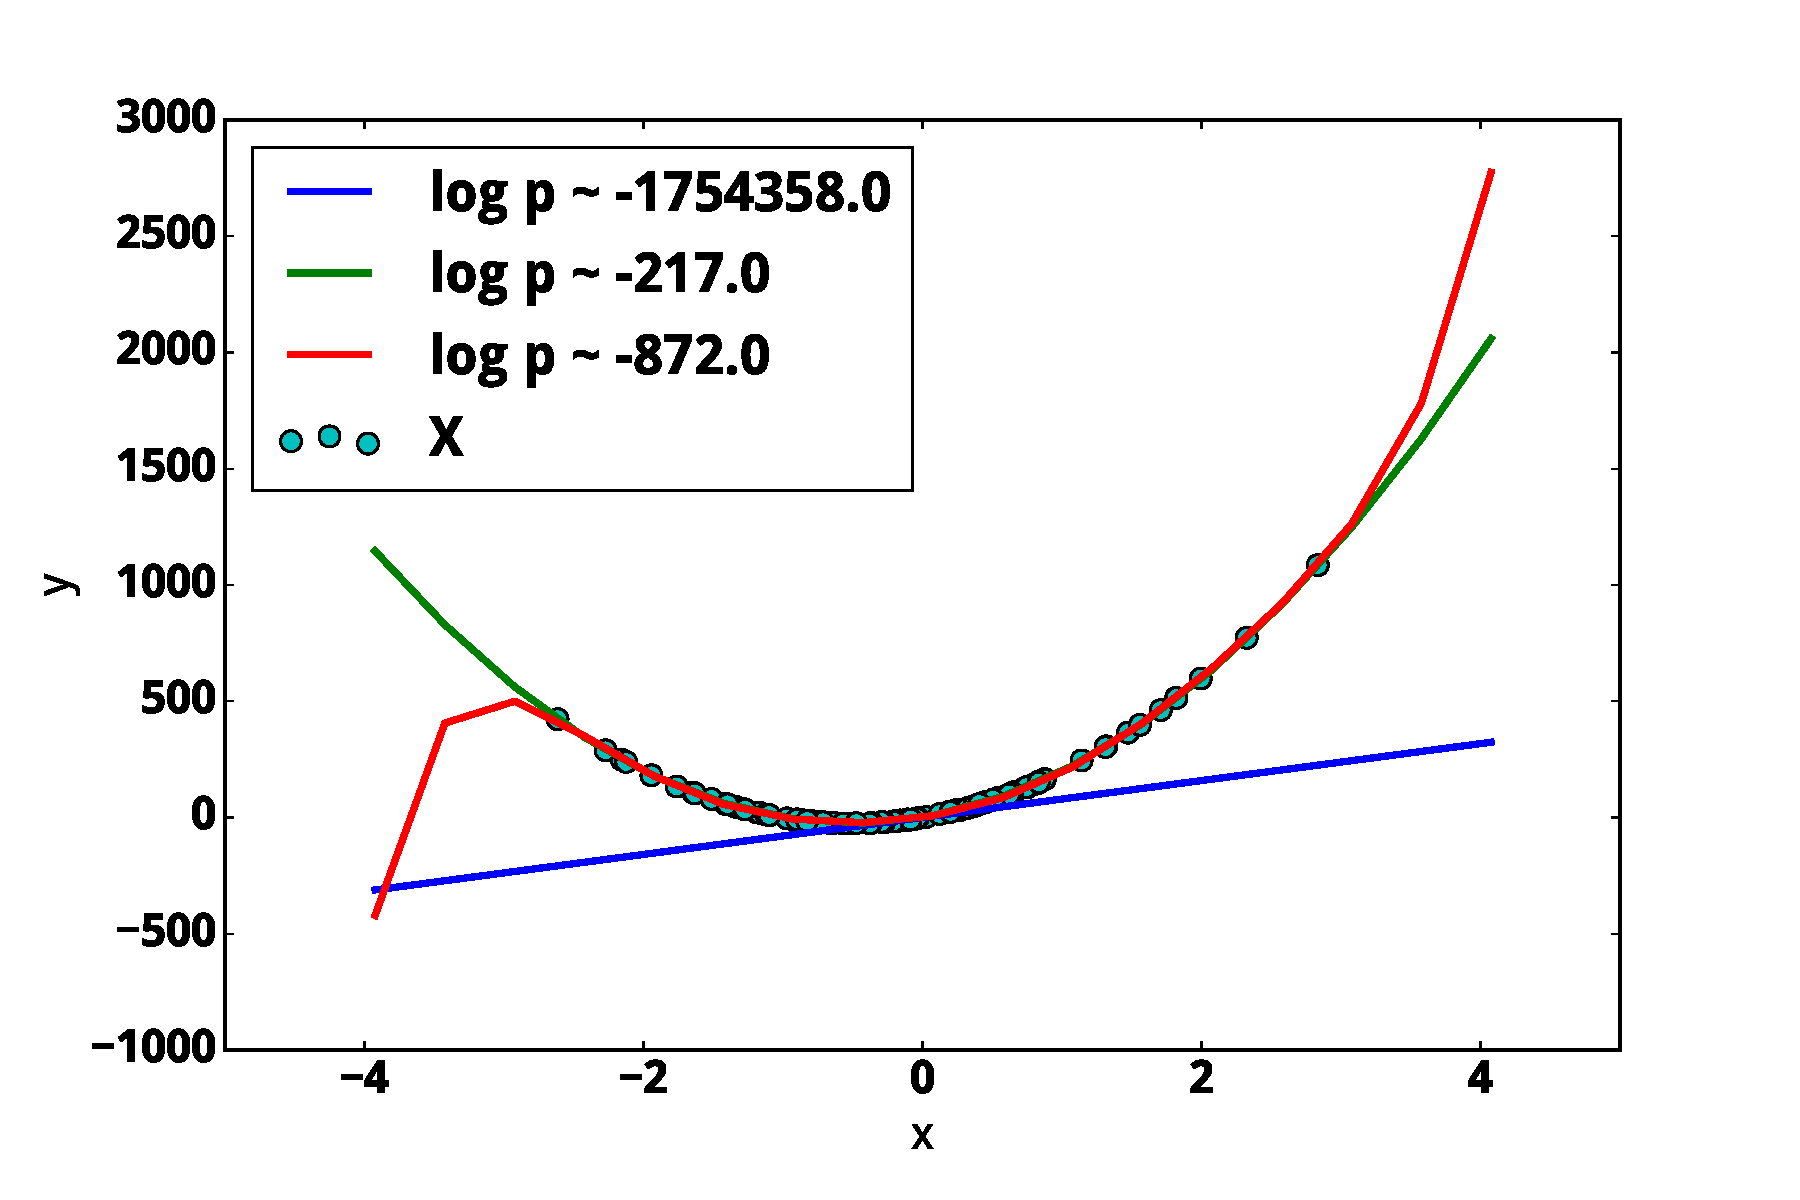
\includegraphics[width=0.4\textwidth]{slide_plots/example.pdf}}

\end{figure}
\end{frame}


\begin{frame}{Выбор оптимальной модели}
\textbf{Основные проблемы выбора оптимальной модели}\\
\begin{itemize}
\item Интеграл правдоподобия невычислим аналитически.
\item Задача оптимизации многоэкстремальна и невыпукла.
\end{itemize}
~\\
\textbf{Требуется}\\ 
Предложить метод поиска субоптимального решения задачи оптимизации, позвяоляюещго проводить оптимизацию в различных режимах:
\begin{itemize}
\item Оптимизация правдоподобия.
\item Последовательное увеличиение сложности модели.
\item Последовательное снижение сложности модели.
\item Полный перебор вариантов структуры модели.
\end{itemize}

\end{frame}       


                                                                                                                                   
                                                                                                                                    

\begin{frame}{Вариационная нижняя оценка правдоподобия}     
\textbf{Правдоподобие модели:}
\[
p(\mathbf{y}|\mathbf{X},\mathbf{A},\mathbf{m}, c_{\text{temp}}) =
\]
\[
 \int_{\mathbf{W}, \boldsymbol{\Gamma} } \textcolor{red}{p(\mathbf{y}|\mathbf{X},\mathbf{W},  \boldsymbol{\Gamma})} \textcolor{blue}{p(\mathbf{W}|\mathbf{A}, \boldsymbol{\Gamma})p(\boldsymbol{\Gamma}|\mathbf{m}, c_{\text{temp}})} d\mathbf{W}d{\boldsymbol{\Gamma}}.                         
\]

Пусть $q$ --- непрерывное распределение.
$$                                                                                                                                              
        \text{log}~p(\mathbf{y}|\mathbf{X},\mathbf{A},\mathbf{m}, c_{\text{temp}}) \geq 
$$          
$$                                                                                                                                              
         \geq  \textcolor{blue}{\int q(\mathbf{W})\text{log}~{p(\mathbf{y} | \mathbf{X}, \mathbf{W}, \boldsymbol{\Gamma}. \mathbf{A}^{-1}, c_{\text{temp}})}d \mathbf{W}d\boldsymbol{\Gamma}} -$$ 
    $$  \textcolor{red}{-\int q(\mathbf{w})\text{log}~\frac{p(\mathbf{w}, \boldsymbol{\Gamma} |\mathbf{A}^{-1}, \mathbf{m}, c_{\text{temp}})}{q(\mathbf{W}, \boldsymbol{\Gamma})}d\mathbf{W}d\boldsymbol{\Gamma}} =$$
$$
\textcolor{blue}{\mathsf{E}_q \text{log}~{p(\mathbf{y} | \mathbf{X}, \mathbf{W}, \boldsymbol{\Gamma}. \mathbf{A}^{-1}, c_{\text{temp}})}} - \textcolor{red}{\text{D}_{KL}(p(\mathbf{w}, \boldsymbol{\Gamma} |\mathbf{A}^{-1}, \mathbf{m}, c_{\text{temp}}) || q(\mathbf{W}, \boldsymbol{\Gamma}))}.
$$ 

\end{frame}      
   


\begin{frame}{ Постановка задачи}
\textcolor{red}{\textbf{TODO: ослабить? Как писать заголовки для этих слайдов?\\}}
\textcolor{red}{\textbf{TODO: Что мы считаем моделью?\\}}

Задан граф $V,E$. \\
Для каждого ребра $(j,k) \in E$ определен вектор \textbf{базовых функций} $\mathbf{g}_{j,k}$ мощностью $K_{j,k}$.\\
Граф $V, E$ со множеством функций $\mathfrak{G} = \{\mathbf{g}_{j,k}\}_{(j,k) \in E}$ называется \textbf{моделью}, если функция, задаваемая рекурсивно как 
\[
    f_j(\mathbf{x}) = \sum_{k \in \text{Adj}(v_j)} <\boldsymbol{\gamma}_{j,k}, \mathbf{g}_{j,k}> (f_{k}(\mathbf{x})), \quad     f_0(\mathbf{x}) = \mathbf{x},
\]
является непрерывной дифференцируемой функцией из $\mathbb{R}^n$ во множество $\mathbb{Y}$ при любых значениях векторов $\boldsymbol{\gamma}$.

Обозначим за вектор \textbf{параметров модели}  $\mathbf{W}$ конкатенацию параметров всех подмоделей $\{f_j\}_{j=1}^{|V|}$.
\end{frame}


\begin{frame}{ Распределение на структуре}
Пусть для каждого ребра $(j,k)$ задан нормированный положительный вектор $\boldsymbol{\gamma}_{j,k} \in \mathbb{R}_{+}^{|K_{j,k}|}$, определяющий веса баховых функций из  $\mathbf{g}(j,k)$.

Будем считать, что вектор $\boldsymbol{\gamma}_{j,k}$ распределен по распределению Gumbel-Softmax:
\[
    p(\boldsymbol{\gamma}) = (K_{j,k}-1)!{c_{\text{temp}}}^{K_{j,k}-1}\left(\prod_{h=1}^{K_{j,k}-1} \alpha_h \boldsymbol{\gamma}_h^{-c_{\text{temp}}-1}\right)\left(\sum_{h=1}^u\alpha_h\boldsymbol{\gamma}_h^{-c_{\text{temp}}}\right),
\] 
где $\alpha_1,\dots,\alpha_h$ --- параметры сдвига распределения, $c_{\text{temp}}$ --- температура распределения. 
\\~\\
Обозначим за \textbf{структуру} модели $\boldsymbol{\Gamma}$ множество всех векторов $\boldsymbol{\gamma}_{j,k}$.\\
Обозначим за $\mathbf{m}$ параметры сдвига всех распределений, соответствующих структуре $\boldsymbol{\Gamma}$.

\end{frame}




\begin{frame}{Вариационный вывод: распределение структурных параметров}
Для каждого элемента структуры $\boldsymbol{\gamma}$ зададим распределение весов базовых функций по распределению Gumbel-Softmax c параметрами $\hat{\alpha}_1, \dots, \hat{\alpha}_u, c$, где параметр $c$ --- общий для всех весов.

Для реализации $h$-й компоненты случайной величины $\boldsymbol{\gamma}$ справедлива следующая формула:
\[
    \hat{\boldsymbol{\gamma}}^h = \text{exp}\left(\text{log}\left(\alpha_h + \text{Gum}_h\right)c^{-1}\right) \sum_{h=1}^l \text{exp}\left(\text{log}\left(\alpha_l + \text{Gum}_l\right)c^{-1}\right),
\]
где $\text{Gum} \sim -\text{log}(-\text{log}~\mathcal{U}(0,1)).$ 
\end{frame}

\iffalse
\begin{frame}{Задача оптимизации}
Пусть параметры распределения распределены нормально:
\[
    p(\mathbf{W}) \sim \mathcal{N}(\mathbf{0}, \mathbf{A}^{-1}).
\]

Требуется найти гиперпараметры модели $\mathbf{A}, \mathbf{m}$ доставляющие максимум правдоподобия модели:
\[
    \argmax_{\mathbf{A}, \mathbf{m}}  p(\mathbf{y}|\mathbf{X},\mathbf{A},\mathbf{m}, c_{\text{temp}}).
\]                                                                                                                            
\textcolor{red}{\textbf{TODO: насколько это формально?\\}}
\begin{block}{Теорема}
При устремлении $c_{\text{temp}}$ к нулю задача становится эквивалентна дискретной задаче оптимизации:
\[
    \argmax_{\mathbf{A}, \{\boldsymbol{\gamma}_{j,k} \in \Delta^{K_{j,k} -1}, (j,k) \in E\}} p(\mathbf{y}|\mathbf{X},\mathbf{A},\mathbf{m}, c_{\text{temp}}) \text{ при }c_{\text{temp}} \to 0,
\]    
где $\Delta^{K_{j,k} -1}$ --- множество векторов, соответствующих вершинам $(K_{j,k}-1)$-сипмлекса.
\end{block}           
\end{frame}  
\fi

    

\begin{frame}{Вариационный вывод: распределение параметров}
Пусть $\mathbf{W} \sim \mathcal{N}(\mathbf{0}, \mathbf{A}^{-1})$ и структура модели $\boldsymbol{\Gamma}$ определена однозначно.

Пусть $q_\mathbf{W} = \mathcal{N}(\boldsymbol{\mu}_q, \mathbf{A}^{-1}_q), \quad \boldsymbol{\theta} =  [\boldsymbol{\mu}_q, \mathbf{A}^{-1}_q].$ \\
Тогда вариационная оценка имеет вид:
$$
\textcolor{blue}{\int_{\mathbf{W}} q(\mathbf{W})\text{log}~{p(\mathfrak{D},\mathbf{W},\mathbf{A}^{-1})} d \mathbf{W}} - \textcolor{red}{D_\text{KL}\bigl(q_\mathbf{W} (\mathbf{W} )|| p (\mathbf{W}|\mathbf{A}^{-1})\bigr)} \simeq
$$
$$
\sum_{i=1}^m \textcolor{blue}{\text{log}~p(\mathbf{x}_i | \mathbf{W}_i)} - \textcolor{red}{D_\text{KL}\bigl(q_\mathbf{W} (\mathbf{W} )|| p (\mathbf{W}|\mathbf{A}^{-1})\bigr)} = -L(\boldsymbol{\theta}, \mathbf{A}^{-1}, \mathfrak{D}),
$$
где $\mathbf{W}_i \sim q_\mathbf{W}$.

Дивергенция $\textcolor{red}{D_\text{KL}\bigl(q_\mathbf{W} (\mathbf{w} )|| p (\mathbf{W}|\mathbf{A}^{-1})\bigr)}$ вычисляется аналитически:
$$
\textcolor{red}{D_\text{KL}\bigl(q_\mathbf{W} (\mathbf{W}) || p (\mathbf{w}|\mathbf{A}^{-1})\bigr)} = \frac{1}{2} \bigl( \text{tr} (\mathbf{A}\mathbf{A}^{-1}_q) + \boldsymbol{\mu}_q^\text{T}\mathbf{A}\boldsymbol{\mu}_q - n +\text{ln}~|\mathbf{A}^{-1}| - \text{ln}~|\mathbf{A}^{-1}_q| \bigr).
$$

\end{frame}

\begin{frame}
\frametitle{Вариационная оценка на основе мультистарта}
$$\text{log}p(\mathbf{y}|\mathbf{X}, \mathbf{A}) \geq \mathsf{E}_{q(\mathbf{W)}}\text{log~}p (\mathbf{y}, \mathbf{W}|\mathbf{X}, \mathbf{A}^{-1}) - \mathsf{E}_{q_{\mathbf{W}}}(-\text{log}(q_\mathbf{W})).$$

\textbf{Теорема [Бахтеев, 2016].}~Пусть $L$ --- функция потерь, градиент которой ---  непрерывно-дифференцируемая функция с константой Липшица $C$. Пусть $\boldsymbol{\theta} = [\mathbf{W}^1,\dots,\mathbf{W}^k]$ ---  начальные приближения оптимизации модели. Пусть $\beta$ --- шаг градиентного спуска, такой что:
\begin{itemize}
\item $\beta<\frac{1}{C}$,
\item $\beta^{(-1)} > \max_{r \in \{1,\dots,k\}}\lambda_\text{max} (\mathbf{H}(\mathbf{W}^r))$.
\end{itemize}
Тогда
\small
\[
	\mathsf{E}_{q^{\tau}_{\mathbf{W}}}(-\text{log}(q^{\tau}_\mathbf{W})) -  \mathsf{E}_{q^{\tau-1}_{\mathbf{W}}}(-\text{log}(q^{\tau-1}_\mathbf{W}))  \sim  \frac{1}{k}\sum_{r=1}^k \bigl(\beta Tr[\mathbf{H}(\mathbf{W}^r)] - \beta^2 Tr[\mathbf{H}(\mathbf{W}^r)\mathbf{H}(\mathbf{w}^r)]  \bigr) + o_{\beta \to 0}(1),
\]
где $\mathbf{H}$ --- гессиан функции потерь $L$, $q^{\tau}_\mathbf{W}$ --- распределение $q^{\tau}_\mathbf{W}$ в момент оптимизации $\tau$.
\end{frame}


\begin{frame}
\frametitle{Вариационная оценка с использованием градиентного спуска}
\footnotesize
Максимизация вариационной оценки эквивалентна минимизации $\text{D}_{\text{KL}}(q(\mathbf{W})||p(\mathbf{W} | \mathfrak{D},\mathbf{A}^{-1}))$.\\
Градиентный спуск не минимизирует $\text{D}_{\text{KL}}(q(\mathbf{W})||p(\mathbf{W} | \mathfrak{D},\mathbf{A}^{-1}))$.
\begin{multicols}{2}

\begin{figure}
\subfloat{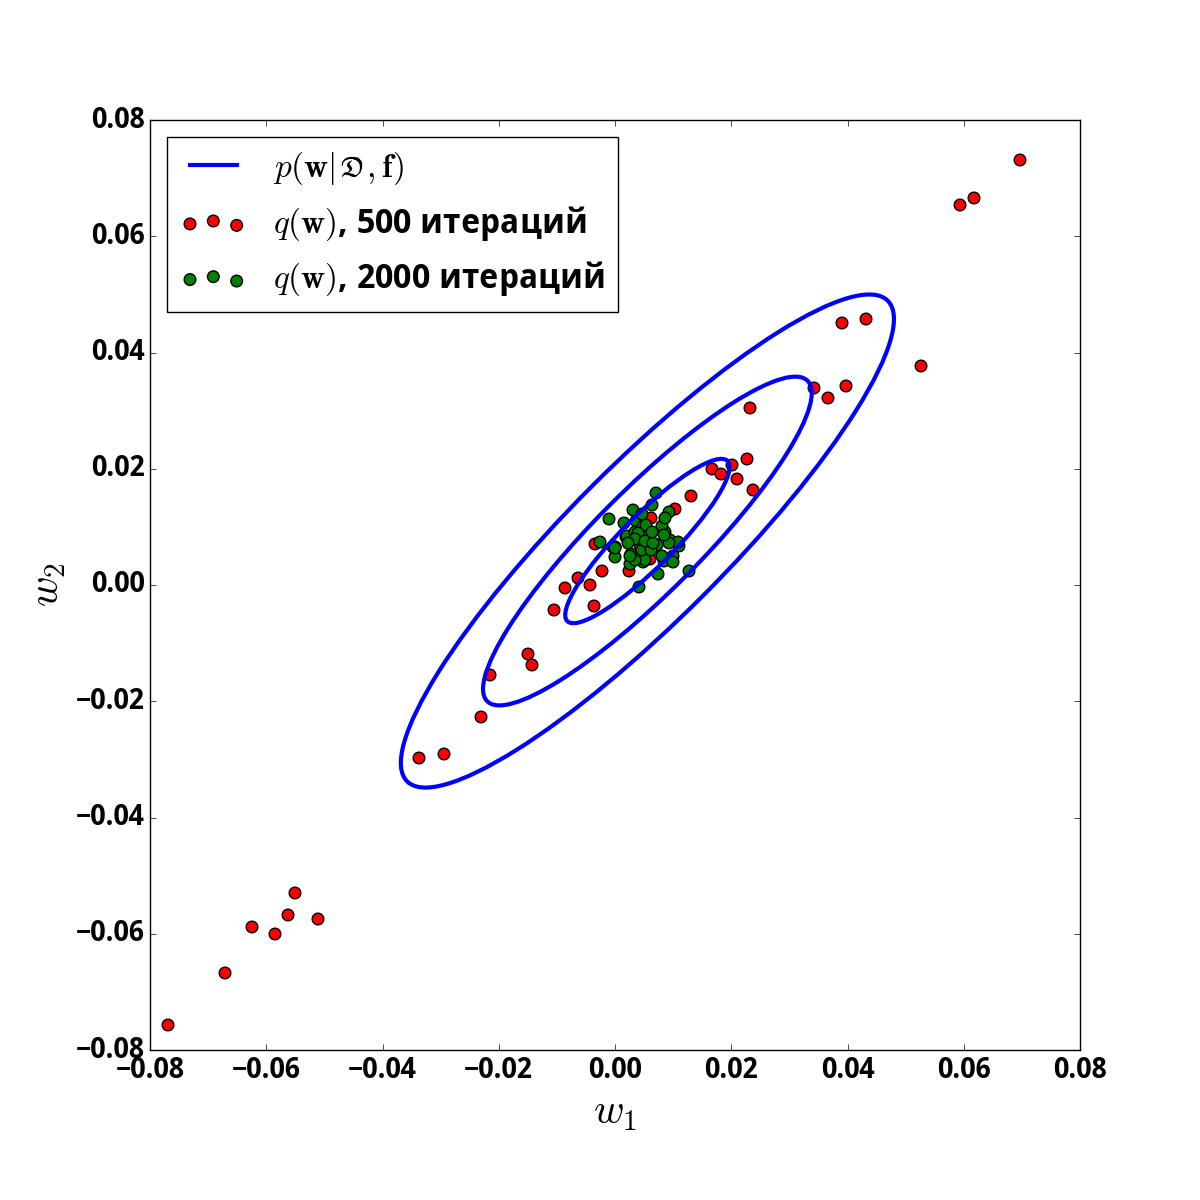
\includegraphics[width=0.38\textwidth]{./slide_plots/sgd_estimate.png}}
\end{figure}

\columnbreak


\begin{figure}
{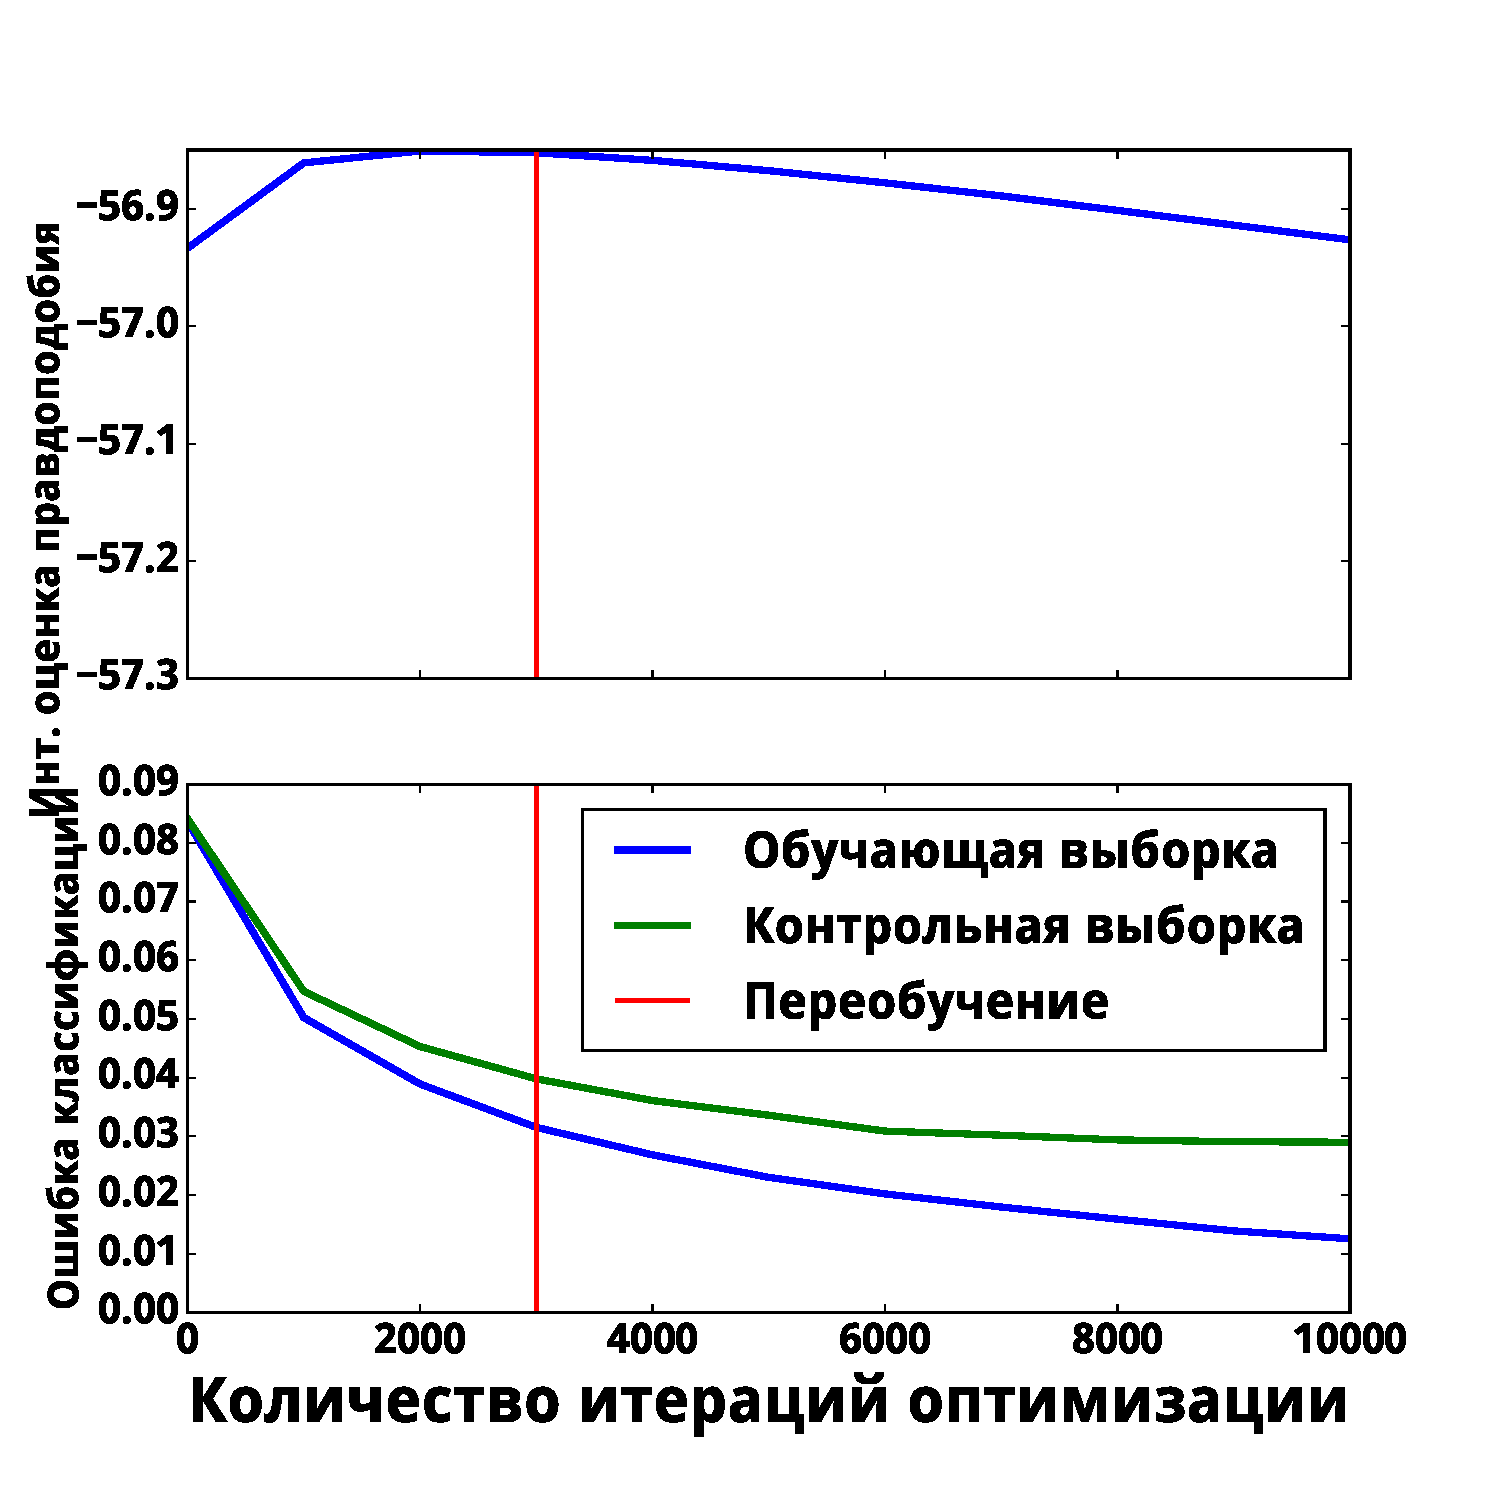
\includegraphics[width=0.38\textwidth]{./slide_plots/sgd_show.pdf}}
\end{figure}
\end{multicols}
\end{frame}


\begin{frame}{Оптимизация параметров вариационного распределения}
\footnotesize
Оптимизацию параметров вариационного распределения будем проводить по следующему функционалу:
\[
L =
\textcolor{blue}{\mathsf{E}_q \text{log}~{p(\mathbf{y} | \mathbf{X}, \mathbf{W}, \boldsymbol{\Gamma}. \mathbf{A}^{-1}, c_{\text{temp}})}} - \textcolor{red}{c_\text{reg}\text{D}_{KL}(p(\mathbf{w}, \boldsymbol{\Gamma} |\mathbf{A}^{-1}, \mathbf{m}, c_{\text{temp}}) || q(\mathbf{W}), q(\boldsymbol{\Gamma}))} \to \max
\]

\begin{block}{Теорема}
Пусть $c_\text{reg} > 0$ .
Тогда функция $L$ сходится по вероятности к вариационной нижней оценке правдоподобия для подвыборки  $\mathfrak{D}$ 
мощностью $c_\text{reg} m$:
$$
L \to^p c_\text{reg} m \int q(\mathbf{W}, \boldsymbol{\Gamma})\text{log}~\frac{p(\mathbf{y}, \mathbf{W}, \boldsymbol{\Gamma}|\mathbf{X},\mathbf{A},\mathbf{m}, c_{\text{temp}})}{q(\mathbf{W}, \boldsymbol{\Gamma})}d\mathbf{W}d\boldsymbol{\Gamma}
$$
\end{block}

\begin{block}{Теорема}
Пусть $c_{\text{reg}}>0.$ При устремлении $c_{\text{temp}}$ к нулю задача становится эквивалентна дискретной задаче оптимизации:
\[
    \argmax_{\mathbf{A}, \{\boldsymbol{\gamma}_{j,k} \in \Delta^{K_{j,k} -1}, (j,k) \in E\}} \textcolor{blue}{\mathsf{E}_q \text{log}~{p(\mathbf{y} | \mathbf{X}, \mathbf{W}, \boldsymbol{\Gamma}. \mathbf{A}^{-1}, c_{\text{temp}})}} - \textcolor{red}{c_\text{reg}\text{D}_{KL}(p(\mathbf{w}, \boldsymbol{\Gamma} |\mathbf{A}^{-1}, \mathbf{m}, c_{\text{temp}}) || q(\mathbf{W}), q(\boldsymbol{\Gamma}))},
\]    
где $\Delta^{K_{j,k} -1}$ --- множество векторов, соответствующих вершинам $(K_{j,k}-1)$-сипмлекса.
\end{block} 

\end{frame}


\begin{frame}{Оптимизация параметров априорного распределения}
Оптимизацию параметров априорного распределения будем проводить по следующему функционалу:
\[
Q = \textcolor{blue}{c_\text{train}\mathsf{E}_q \text{log}~{p(\mathbf{y} | \mathbf{X}, \mathbf{W}, \boldsymbol{\Gamma}. \mathbf{A}^{-1}, c_{\text{prior}})}}
 - \textcolor{red}{c_\text{prior}\text{D}_{KL}(p(\mathbf{W}, \boldsymbol{\Gamma} |\mathbf{A}^{-1}, \mathbf{m}, c_{\text{temp}}) || q(\mathbf{W}, \boldsymbol{\Gamma}))} -\]
\[
 - \textcolor{OliveGreen}{c_{\text{comb}}\sum_{p' \in \mathbf{P}} \text{D}_{KL}(\boldsymbol{\Gamma} | p')} \to \max, 
\]
где $\mathbf{P}$ --- множество (возможно пустое) распределений на структуре модели.
\end{frame}

\begin{frame}{Общая задача оптимизации}
Общая задача оптимизации --- двухуровневая:
\[
\hat{\mathbf{A}}, \hat{\mathbf{m}} = \argmax_{\mathbf{A}, \mathbf{m}} Q = 
\]
\[
= \textcolor{blue}{c_\text{train}\mathsf{E}_{\hat{q}} \text{log}~{p(\mathbf{y} | \mathbf{X}, \mathbf{W}, \boldsymbol{\Gamma}. \mathbf{A}^{-1}, c_{\text{prior}})}}
 - \textcolor{red}{c_\text{prior}\text{D}_{KL}(p(\mathbf{W}, \boldsymbol{\Gamma} |\mathbf{A}^{-1}, \mathbf{m}, c_{\text{temp}}) || \hat{q}(\mathbf{W}, \boldsymbol{\Gamma}))} -\]
\[
 - \textcolor{OliveGreen}{c_{\text{comb}}\sum_{p' \in \mathbf{P}} \text{D}_{KL}(\boldsymbol{\Gamma} | p')}, 
\]
при 
\[
\hat{q} = \argmax_{q} L = 
\textcolor{blue}{\mathsf{E}_q \text{log}~{p(\mathbf{y} | \mathbf{X}, \mathbf{W}, \boldsymbol{\Gamma}. \mathbf{A}^{-1}, c_{\text{temp}})}} - \textcolor{red}{c_\text{reg}\text{D}_{KL}(p(\mathbf{w}, \boldsymbol{\Gamma} |\mathbf{A}^{-1}, \mathbf{m}, c_{\text{temp}}) || q(\mathbf{W}), q(\boldsymbol{\Gamma}))}
\]

\end{frame}


\begin{frame}{Оператор оптимизации}
Обозначим за $\mathbf{h}$ гиперпараметры $\mathbf{A}, \mathbf{m}$.\\
Обозначим за $\boldsymbol{\theta}$ параметры распределений $q_{\mathbf{W}}, q_{\boldsymbol{\Gamma}}$.

\begin{block}{Определение}
Оператором $T$ назовем оператор стохастического градиентного спуска, производящий $\eta$ шагов оптимизации:
\begin{equation}
\label{eq:gd}
	 \hat{\boldsymbol{\theta}} = T \circ T \circ \dots \circ T(\boldsymbol{\theta}_0, \mathbf{A}^{-1}) = T^\eta(\boldsymbol{\theta}_0, \mathbf{A}^{-1}),
\end{equation}
где 
$$
	T(\boldsymbol{\theta}, \mathbf{A}^{-1}) =\boldsymbol{\theta} - \beta \nabla L(\boldsymbol{\theta}, \mathbf{A}^{-1})|_{\hat{\mathfrak{D}}}, 
$$
$\gamma$ --- длина шага градиентного спуска, $\boldsymbol{\theta}_0$ --- начальное значение параметров $\boldsymbol{\theta}$, $\hat{\mathfrak{D}}$ --- случайная подвыборка исходной выборки $\mathfrak{D}$.
\end{block}

начальное значение параметров $\boldsymbol{\theta}$.


\end{frame}

\begin{frame}{Оптимизация гиперпараметров}

Перепишем итоговую задачу оптимизации:
\[
	\hat{\mathbf{h}} = \argmax_{\mathbf{h}} Q( T^\eta(\boldsymbol{\theta}_0, \mathbf{A}^{-1})),
\]
где $\boldsymbol{\theta}_0$ --- н
\begin{block}{Утверждение, Luketina et al., 2016}
Пусть функции $L$ и $Q$ являются дважды дифференцируемыми и выпуклыми. 
Пусть гессиан функции функции $L$ можно аппроксимировать единичной матрицей:
\[
    \mathbf{H}(L, \boldsymbol{\theta}) \approx \mathbf{I}.
\]
Тогда допустима следующая оптимизация гиперпараметров:
\[
    \mathbf{h}' = \mathbf{h} - \beta^{h} \nabla_{\mathbf{h}} Q(T(\boldsymbol{\theta}), \mathbf{h}),
\]
где $\beta^{h}$ --- шаг оптимизации гиперпараметров.
\end{block}
\end{frame}


\begin{frame}{Оптимизация гиперпараметров: пример}
\begin{multicols}{2}
\begin{figure}[h]
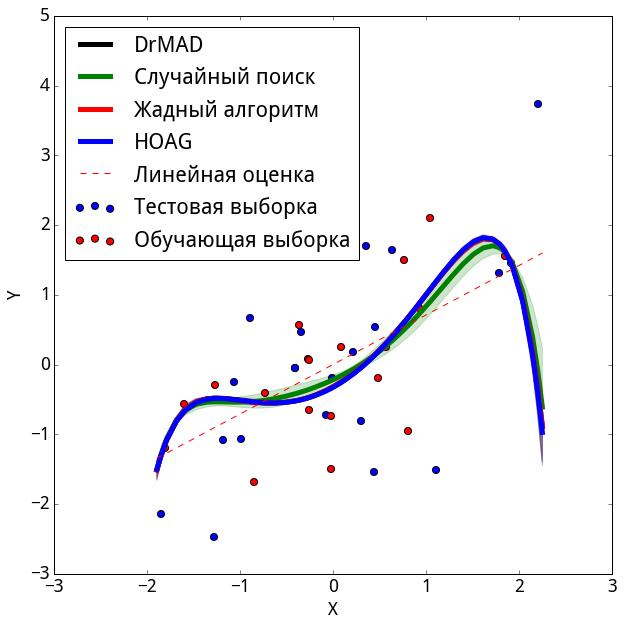
\includegraphics[width=0.4\textwidth]{./slide_plots/poly_cv.png}
\caption*{Кросс-Валидация}
\end{figure}

\begin{figure}[h]
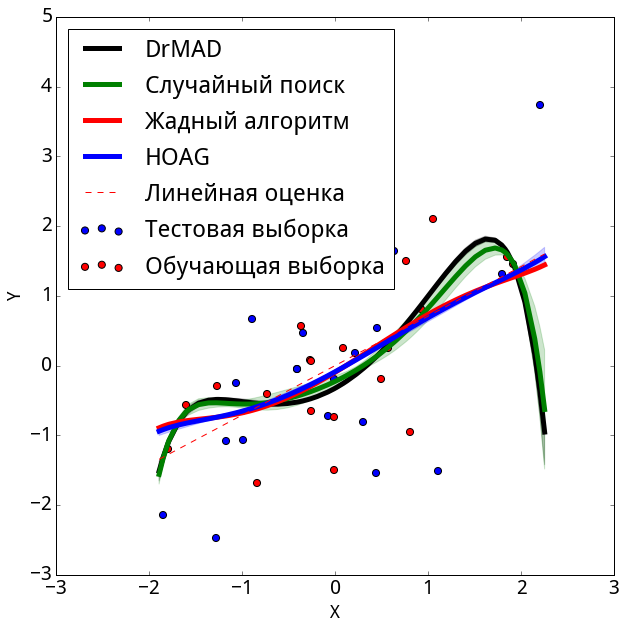
\includegraphics[width=0.4\textwidth]{./slide_plots/poly_var.png}
\caption*{Вариационная оценка}
\end{figure}
\end{multicols}

\end{frame}
\begin{frame}{Оптимизация правдоподобия модели}
\begin{block}{Теорема}
Пусть существуют параметры распределения $q(\mathbf{W}, \boldsymbol{\Gamma})$, такие что $\text{D}_\text{KL}(q(\mathbf{W}, \boldsymbol{\Gamma})|p(\mathbf{W},  \boldsymbol{\Gamma}| \mathbf{y}, \mathbf{X}, \mathbf{A}, \mathbf{m}, c_\text{temp})) = 0$.\\
Тогда двухуровневая задача оптимизация эквивалентна исходной задаче оптимизации правдоподобия модели:
$$\argmax_{\mathbf{A}, \mathbf{m}}  p(\mathbf{y}|\mathbf{X},\mathbf{A},\mathbf{m}, c_{\text{temp}})$$ 
при $c_{\text{reg}} = c_{\text{prior}} = c_{\text{train}} = 1, c_{\text{comb}} = 0$. 
\end{block}
~\\
Обозначим за $F(c_{\text{reg}}, c_{\text{train}}, c_{\text{prior}}, c_{\text{comb}}, \mathbf{P}, c_{\text{temp}})$ множество экстремумов функции $L$ при решении задачи двухуровневой оптимизации.
\end{frame}


\begin{frame}{Параметрическая сложность}
\footnotesize
Назовем \textbf{параметрической сложностью модели} наименьшую дивергенцию между априорным распределением параметров и вариационным распредеделением параметров:
\[
    C_\text{param} = \min_{\mathbf{A}, \mathbf{m}} \text{D}_\text{KL}(q(\mathbf{W}, \boldsymbol{\Gamma})||p(\mathbf{W}, \boldsymbol{\Gamma}|\mathbf{A}, \mathbf{m}, c_\text{temp})).
\]
\textcolor{red}{\textbf{TODO: надо ли про bits-back?\\}}
\begin{block}{Теорема}
Пусть $f \in F(1, 1, c_{\text{prior}}, 0, \{\},  c_{\text{temp}} )$.
При устремлении $ c_{\text{prior}}$ к бесконечности параметрическая сложность модели $f$ устремляется к нулю.
\[
    \lim_{c_{\text{prior}} \to \infty} C_{\text{param}}(f) = 0
\]
\end{block}

\begin{block}{Теорема}
Пусть $f_1 \in F(1, 1, c_{\text{prior}}, 0, \{\},  c_{\text{temp}} ), f_2 \in F(1, 1, c_{\text{prior}}, 0, \{\},  c_{\text{temp}}' )$, $c_{\text{prior}} < c_{\text{prior}}'$.
Пусть вариационные параметры моделей $f_1$ и $f_2$ лежат в области $\mathsf{U}$, в которой соответствующие функции $L$ и $Q$ являются локально-выпуклыми. 
Тогда модель $f_1$ имеет параметрическую сложность, не большую чем у $f_2$.
\[
    C_\text{param}(f_1) \leq C_\text{param}(f_2).
\]
\end{block}


\end{frame}

\begin{frame}{Структурная сложность}
\footnotesize
Назовем \textbf{структурной сложностью модели} энтропию вариационного распределения структуры модели:
\[
    C_\text{struct} = -\mathsf{E}_{q_{\boldsymbol{\Gamma}}} \text{log}~q_{\boldsymbol{\Gamma}}(\boldsymbol{\Gamma}).
\]
\begin{block}{Теорема}
Пусть $f \in F(c_{\text{reg}}, c_{\text{train}},  c_{\text{prior}}, 0, \{\},  c_{\text{temp}} )$.\\
При устремлении $ c_{\text{temp}}$ к нулю структурная сложность модели $f$ устремляется к нулю.
\[
    \lim_{c_{\text{temp}} \to \infty} C_\text{struct}(f) = 0
\]
\end{block}

\begin{block}{Теорема}
Пусть $f_1 \in F(c_{\text{reg}}, c_{\text{train}},  c_{\text{prior}}, 0, \{\},  c_{\text{temp}}), f_2 =  \in \lim_{c_{\text{temp}}' \to \infty} F(c_{\text{reg}}, c_{\text{train}},  c_{\text{prior}}, 0, \{\},  c_{\text{temp}'})$.
Пусть вариационные параметры моделей $f_1$ и $f_2$ лежат в области $U$, в которой соответствующие функции $L$ и $Q$ являются локально-выпуклыми. 
Тогда разница структурных сложностей моделей ограничена выражением:
\[
    C_\text{struct}(f_1)  - C_\text{struct}(f_2) \leq \textcolor{blue}{\mathsf{E}_q \text{log}~{p(\mathbf{y} | \mathbf{X}, \mathbf{W}, \boldsymbol{\Gamma}. \mathbf{A}^{-1}, c_{\text{temp}})}} - \textcolor{blue}{\mathsf{E}_q' \text{log}~{p(\mathbf{y} | \mathbf{X}, \mathbf{W}, \boldsymbol{\Gamma}. \mathbf{A}^{-1}, c_{\text{temp}})}}.
\]
\end{block}

% Схема доказательства:
% расписываем неравенства вида: L_1 - DKL(q_1|p1) <L_2 - DKL(q_2|p1)
% Замечаем, что при стремлении к бесконечности гумбель превращается в равномерное
% выражаем все в равномерном
% замечаем, что D_KL = Entropy + const для равномерного
% все
\end{frame}


\begin{frame}{Полный перебор}
Рассмотрим последовательность $N = \prod_{(j,k) \in E} K_{j,k}$ моделей, полученных в ходе оптимизаций вида:
$$f_1 \in F(c_{\text{reg}}, 0, 0, \{\}, 0,  c_{\text{temp}}),$$
$$f_2 \in F(1, 0, 0, \{q_1(\boldsymbol{\Gamma})\}, 0,  c_{\text{temp}}), q_1 \in f_1,$$
$$f_3 \in F(1, 0, 0, \{q_1(\boldsymbol{\Gamma}), q_2(\boldsymbol{\Gamma})\}, 0,  c_{\text{temp}}), q_2 \in f_2.$$

\textcolor{red}{\textbf{TODO: формализовать что такое $q_1, q_2$\\}}

\begin{block}{Теорема}
Вариационные распределения структур $q_{\boldsymbol{\Gamma}}$ последовательности $\mathfrak{F} = \{\lim_{c_{\text{temp}} \to 0} f_1, \dots, \lim_{c_{\text{temp}} \to 0} f_N\}$ вырождаются в дельта-функции вида $\delta(\hat{\Gamma})$, где $\hat{\Gamma}$ --- точка на декартовом произведении вершин симплексов структуры модели.

Вариационные распределения последовательности $\mathfrak{F}$ проходят все возможные комбинации структур модели.
\textcolor{red}{\textbf{TODO: пояснить про дискретность структуры?\\}}
\end{block}
\end{frame}


\begin{frame}{Заключение}
???

\end{frame}

\appendix
\bgroup
\setbeamercolor{background canvas}{bg=black}
\begin{frame}[plain, noframenumbering]
\end{frame}
\egroup



\begin{frame}[plain, noframenumbering]{Исследование основывается на следующих работах}
\begin{itemize}
\item Graves A. Practical variational inference for neural networks //Advances in Neural Information Processing Systems. – 2011
\item  Maclaurin D., Duvenaud D., Adams R. Gradient-based hyperparameter optimization through reversible learning //International Conference on Machine Learning. – 2015
\item  Luketina J. et al. Scalable gradient-based tuning of continuous regularization hyperparameters //International Conference on Machine Learning. - 2016
\item J. Fu et al., DrMAD: Distilling Reverse-Mode Automatic Differentiation for Optimizing
Hyperparameters of Deep Neural Networks // IJCAI - 2016
\item Pedregosa F. Hyperparameter optimization with approximate gradient //International Conference on Machine Learning. – 2016. –
\end{itemize}
\end{frame}



\end{document}
